\documentclass{article}

\usepackage{subcaption}
\usepackage[labelformat=parens,labelsep=quad,skip=3pt]{caption}
\usepackage{graphicx}
\usepackage{geometry}

%\geometry{top=0.1in, left=0.1in, right=0.1in, bottom=0.1in}

\usepackage{array}
\usepackage{makecell}
\usepackage{tabularx}
\usepackage[dvipsnames]{xcolor}
\usepackage{amssymb}
\renewcommand{\tabularxcolumn}[1]{m{#1}}

%\pdfpageheight=5in
%\pdfpagewidth=7.2in

\begin{document}
	\section{Single Subject Estimates}
	\begin{tabularx}{7in}{|m{1em}|X|X|X|X|}
		\hline
		& \multicolumn{1}{c|}{Visual Cue} & \multicolumn{1}{c|}{Tongue} & \multicolumn{1}{c|}{Right Foot} & \multicolumn{1}{c|}{Right Hand} \\ \hline
		\rotatebox{90}{\textbf{Bayesian GLM}}& 
		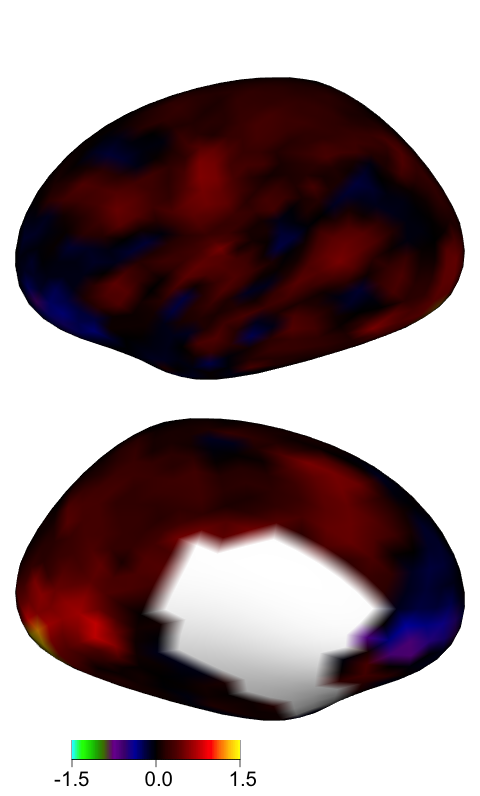
\includegraphics[width=1.5in]{plots/601_single_subject_Bayes_visual_cue.png} &
		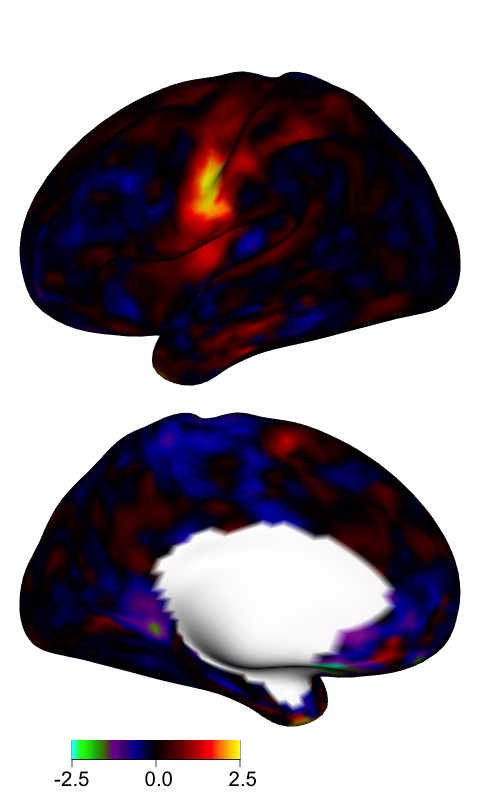
\includegraphics[width=1.5in]{plots/601_single_subject_Bayes_tongue.png} &
		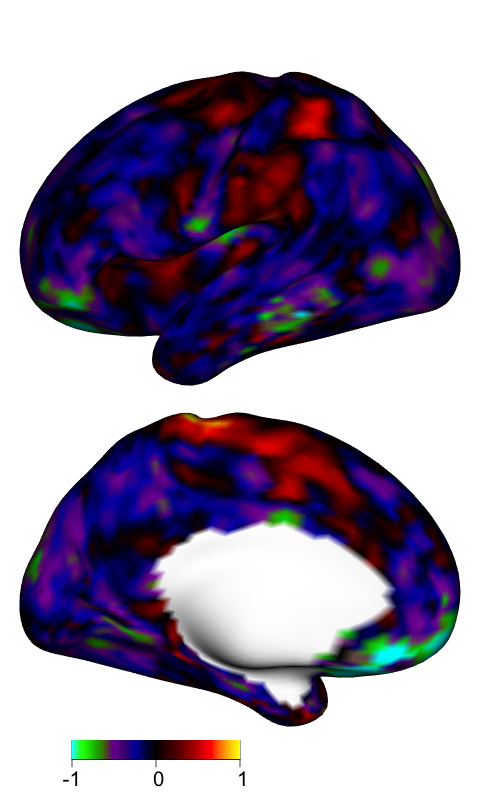
\includegraphics[width=1.5in]{plots/601_single_subject_Bayes_right_foot.png} &
		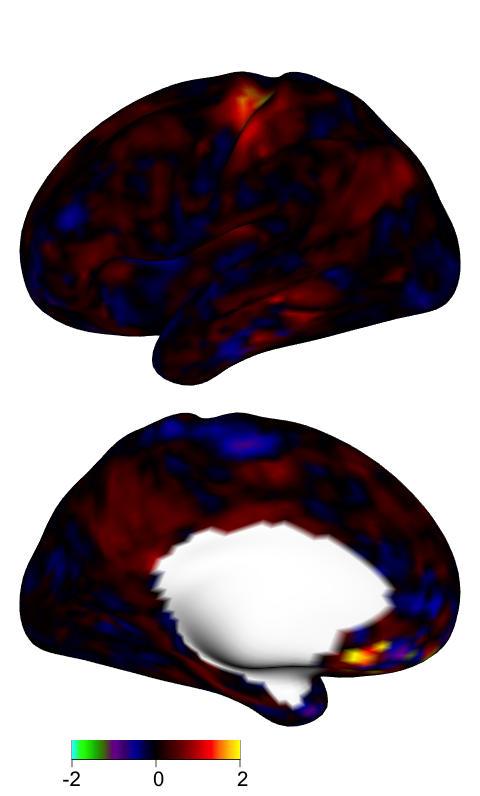
\includegraphics[width=1.5in]{plots/601_single_subject_Bayes_right_hand.png} \\ \hline
		\rotatebox{90}{\textbf{Classical GLM}} & 
		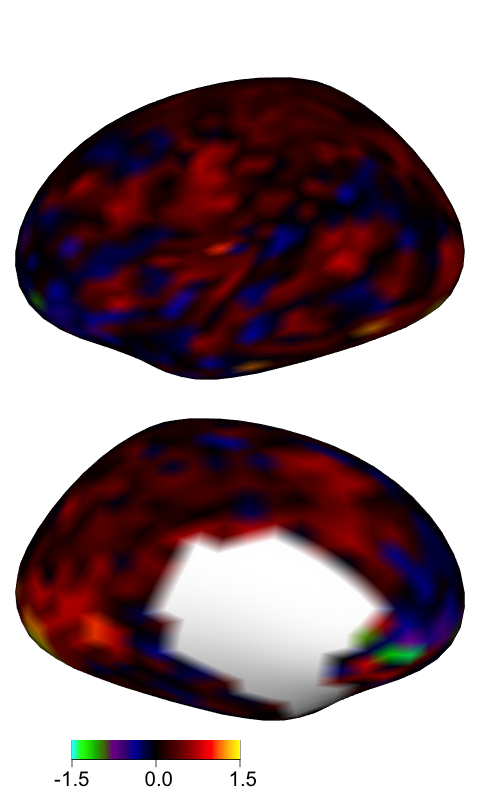
\includegraphics[width=1.5in]{plots/601_single_subject_classical_visual_cue.png} &
		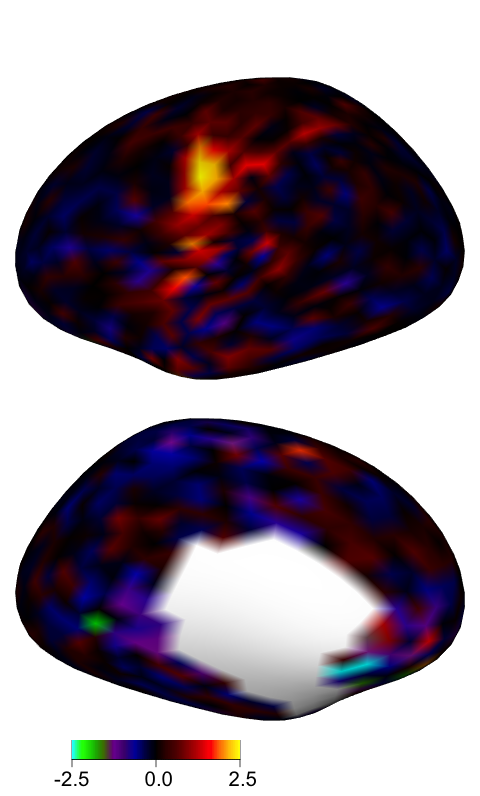
\includegraphics[width=1.5in]{plots/601_single_subject_classical_tongue.png} &
		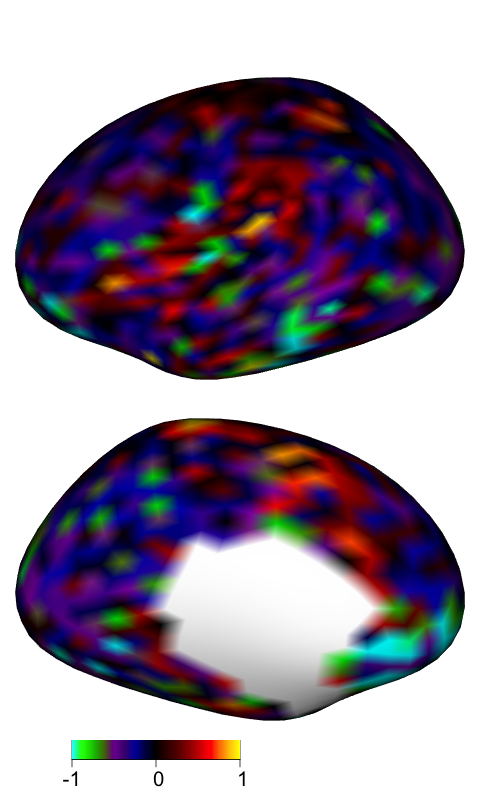
\includegraphics[width=1.5in]{plots/601_single_subject_classical_right_foot.png} &
		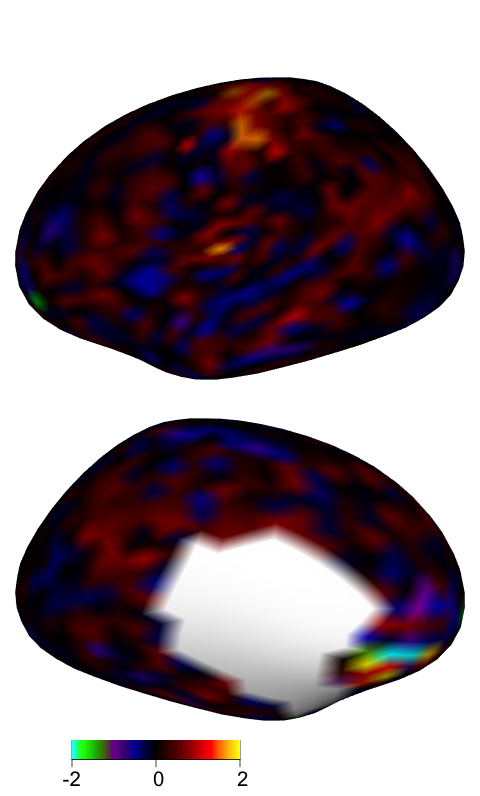
\includegraphics[width=1.5in]{plots/601_single_subject_classical_right_hand.png} \\ \hline
	\end{tabularx}
	
	\newpage
	
	\section{Group Estimates}
	\begin{tabularx}{7in}{|m{1em}|X|X|X|X|}
		\hline
		& \multicolumn{1}{c|}{Visual Cue} & \multicolumn{1}{c|}{Tongue} & \multicolumn{1}{c|}{Right Foot} & \multicolumn{1}{c|}{Right Hand} \\ \hline
		\rotatebox{90}{\textbf{Bayesian GLM}}& 
		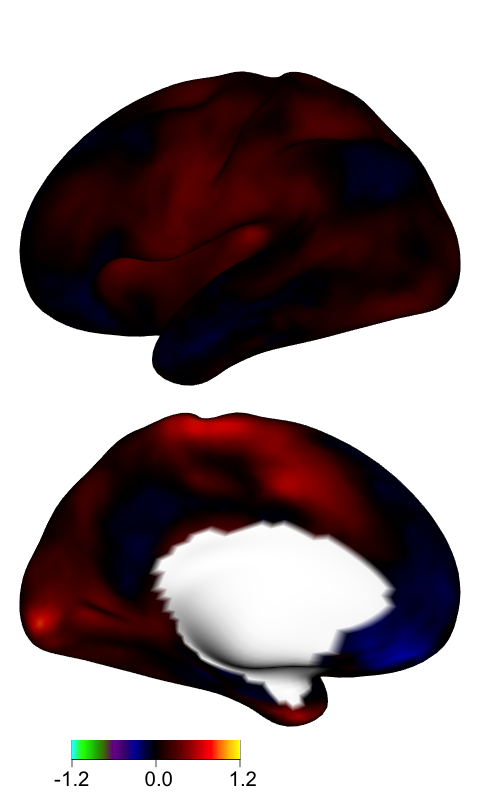
\includegraphics[width=1.5in]{plots/601_group_Bayes_visual_cue.png} &
		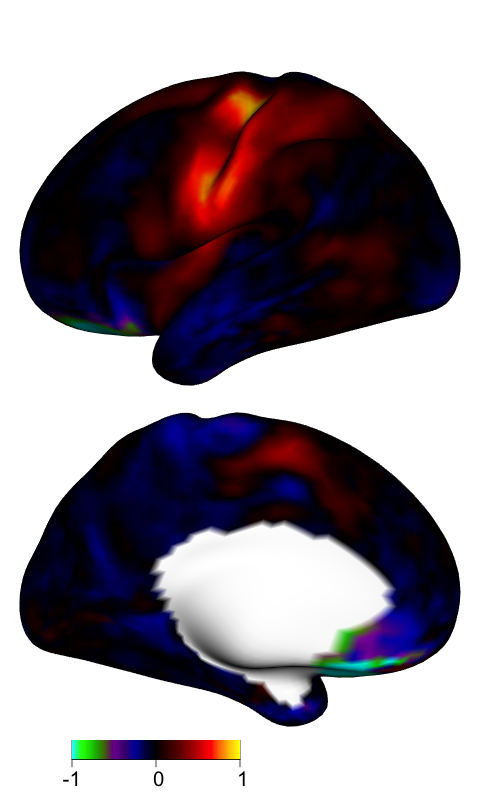
\includegraphics[width=1.5in]{plots/601_group_Bayes_tongue.png} &
		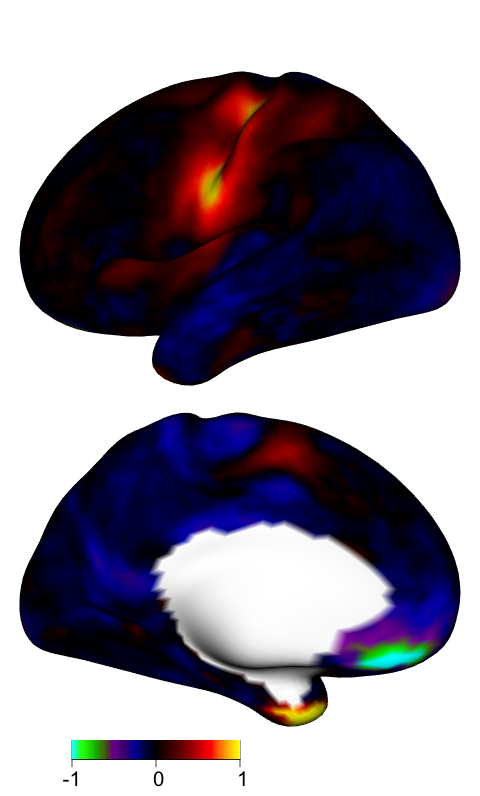
\includegraphics[width=1.5in]{plots/601_group_Bayes_right_foot.png} &
		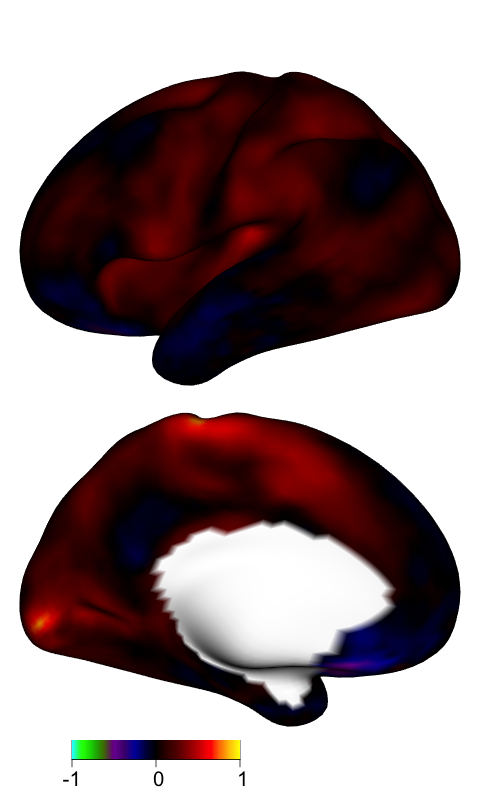
\includegraphics[width=1.5in]{plots/601_group_Bayes_right_hand.png} \\ \hline
		\rotatebox{90}{\textbf{Classical GLM}} & 
		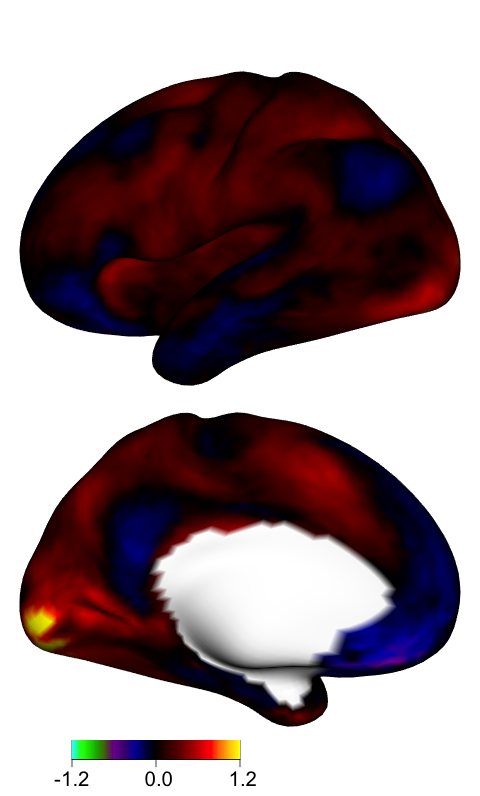
\includegraphics[width=1.5in]{plots/601_group_classical_visual_cue.png} &
		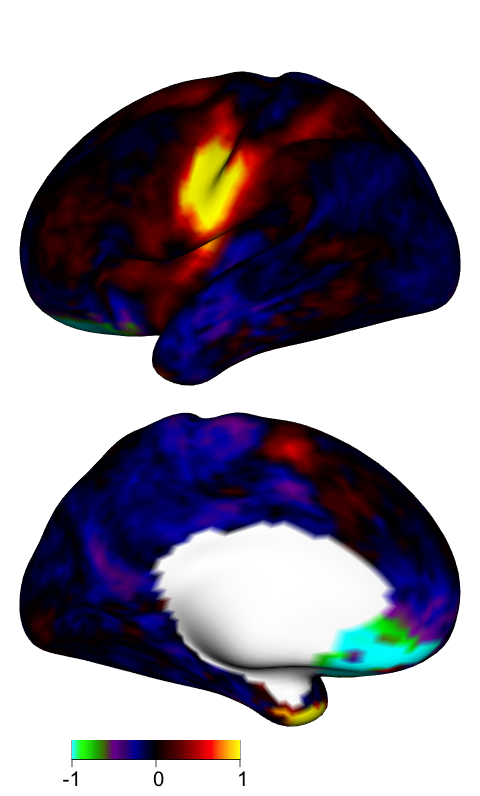
\includegraphics[width=1.5in]{plots/601_group_classical_tongue.png} &
		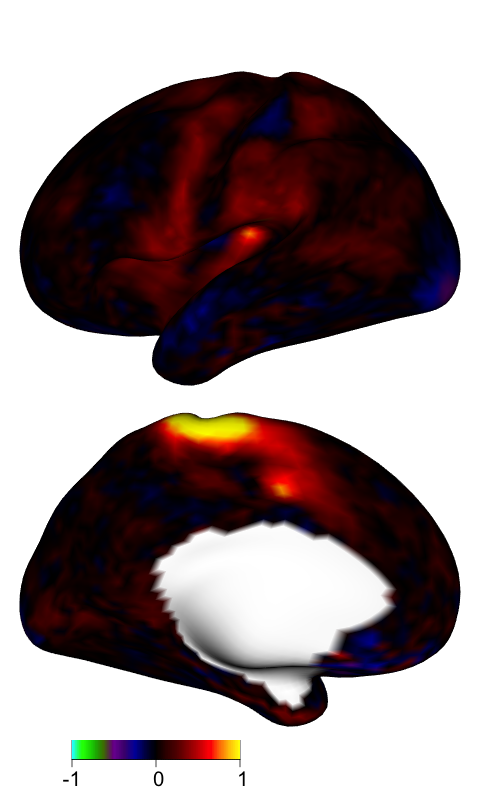
\includegraphics[width=1.5in]{plots/601_group_classical_right_foot.png} &
		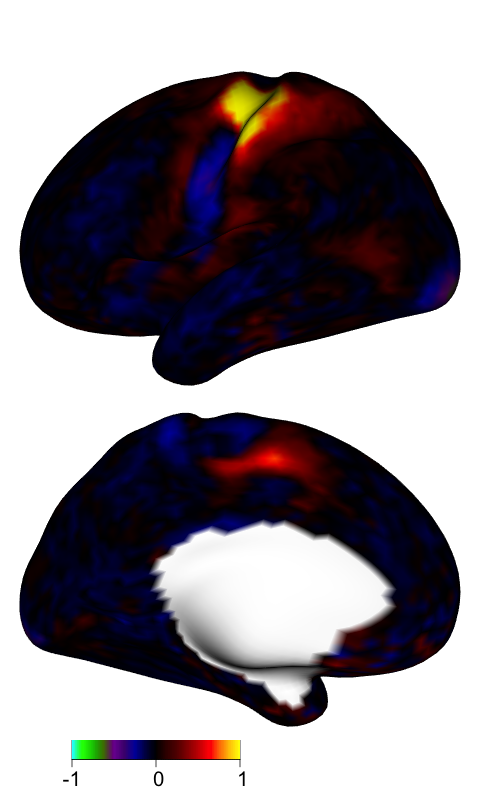
\includegraphics[width=1.5in]{plots/601_group_classical_right_hand.png} \\ \hline
	\end{tabularx}

	\newpage

	\section{Activation}
	\begin{tabularx}{7in}{|m{1em}|X|X|X|X|}
		\hline
		& \multicolumn{1}{c|}{Visual Cue} & \multicolumn{1}{c|}{Tongue} & \multicolumn{1}{c|}{Right Foot} & \multicolumn{1}{c|}{Right Hand} \\ \hline
		\rotatebox{90}{\textbf{Bayesian GLM}}& 
		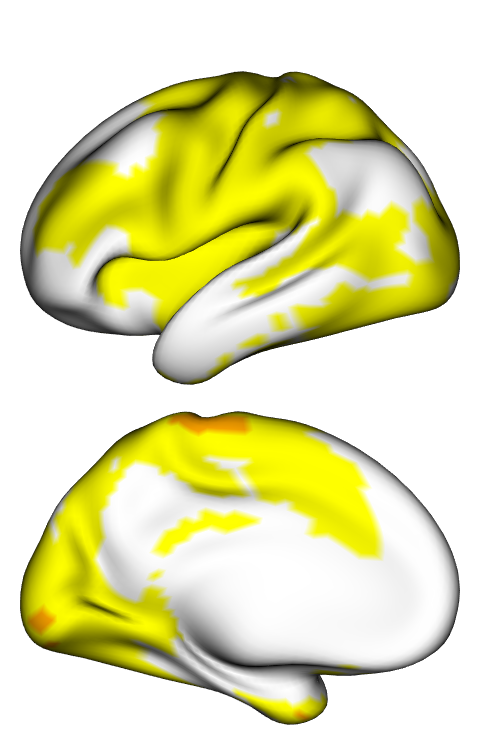
\includegraphics[width=1.5in]{plots/603_visual_cue_activation_map.png} &
		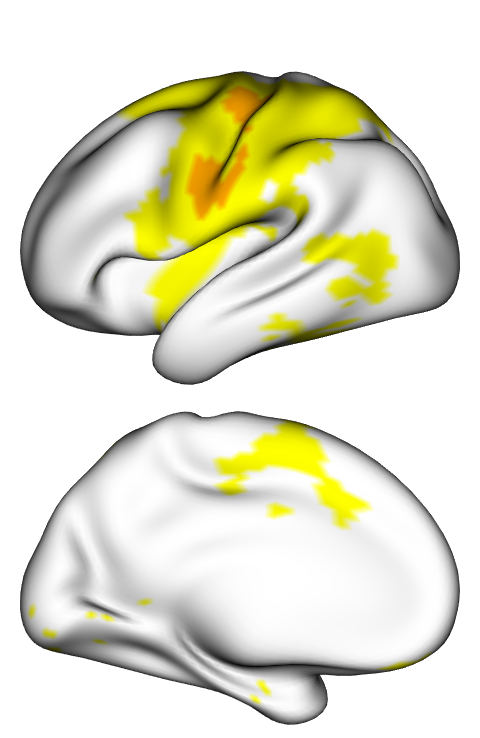
\includegraphics[width=1.5in]{plots/603_tongue_activation_map.png} &
		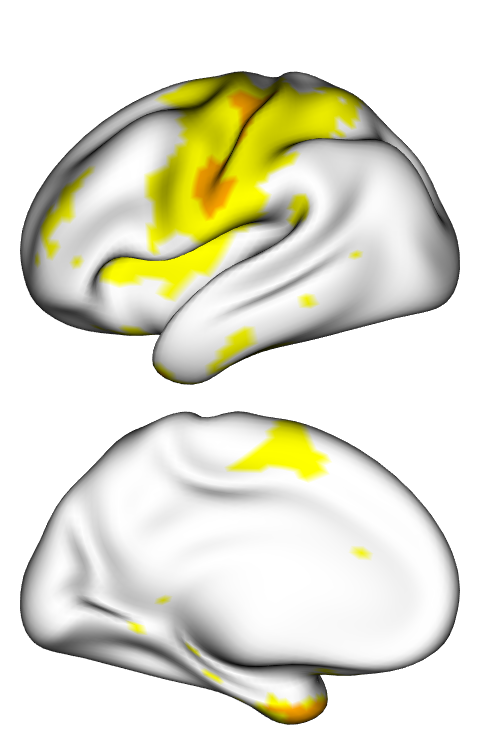
\includegraphics[width=1.5in]{plots/603_foot_activation_map.png} &
		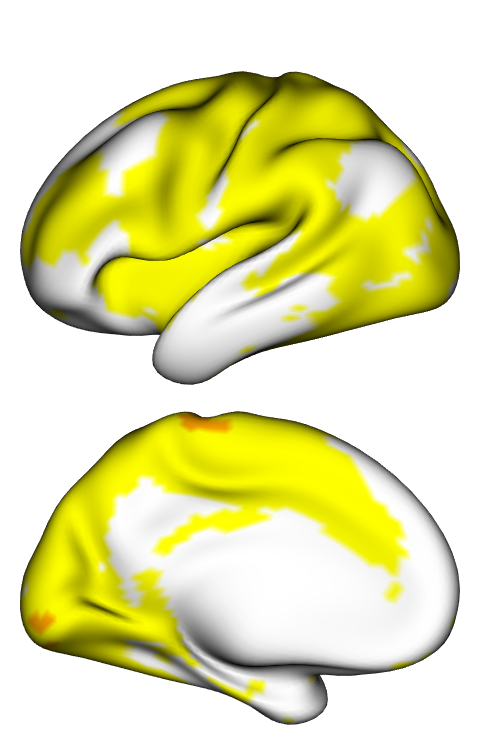
\includegraphics[width=1.5in]{plots/603_hand_activation_map.png} \\ \hline
		\multicolumn{2}{c}{} & \multicolumn{2}{c}{$\gamma = $ \textcolor{yellow}{$\blacksquare$} $0\%$ \textcolor{orange}{$\blacksquare$} $0.5\%$ } & \multicolumn{1}{c}{} \\ \hline
		\rotatebox{90}{\textbf{Classical GLM}} & 
		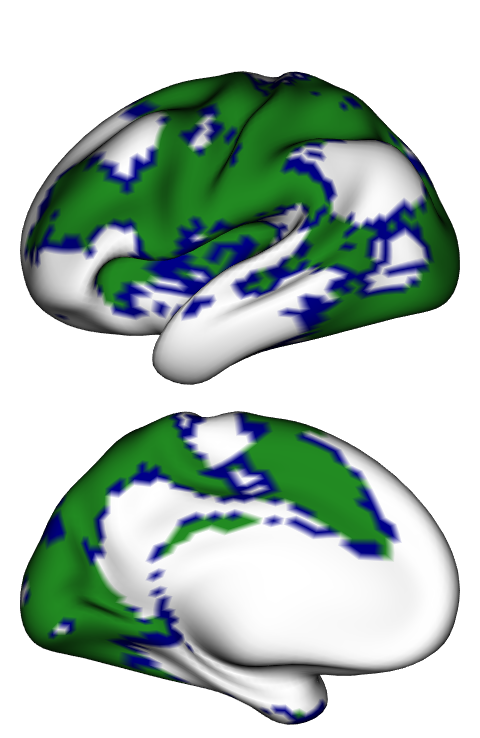
\includegraphics[width=1.5in]{plots/604_visual_cue_classical_activation_map.png} &
		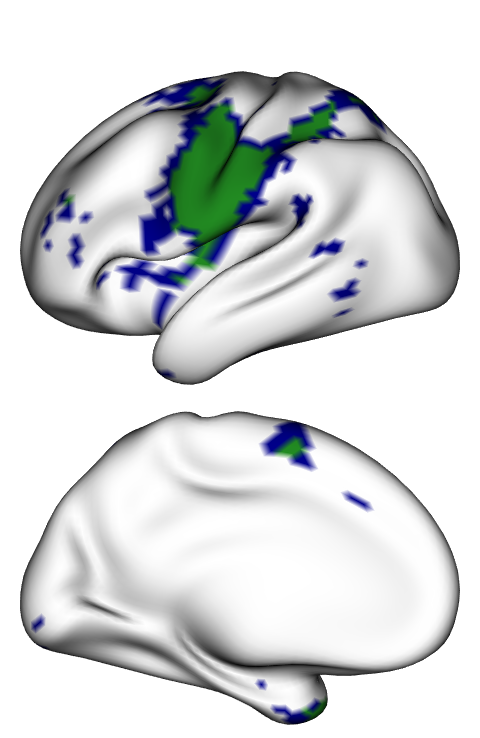
\includegraphics[width=1.5in]{plots/604_tongue_classical_activation_map.png} &
		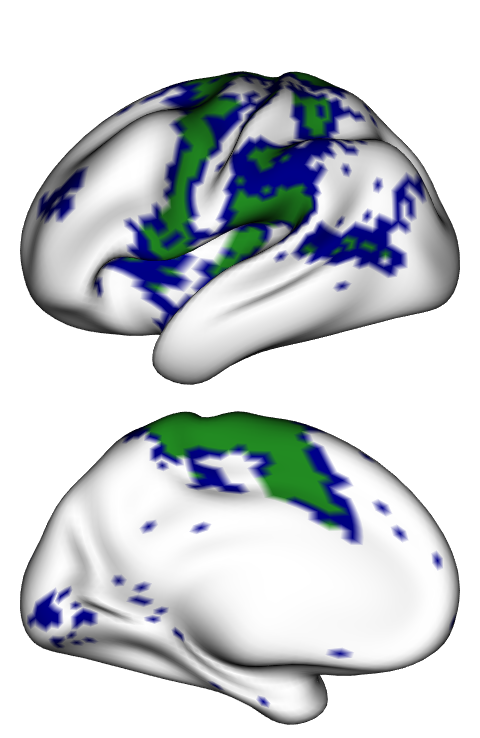
\includegraphics[width=1.5in]{plots/604_foot_classical_activation_map.png} &
		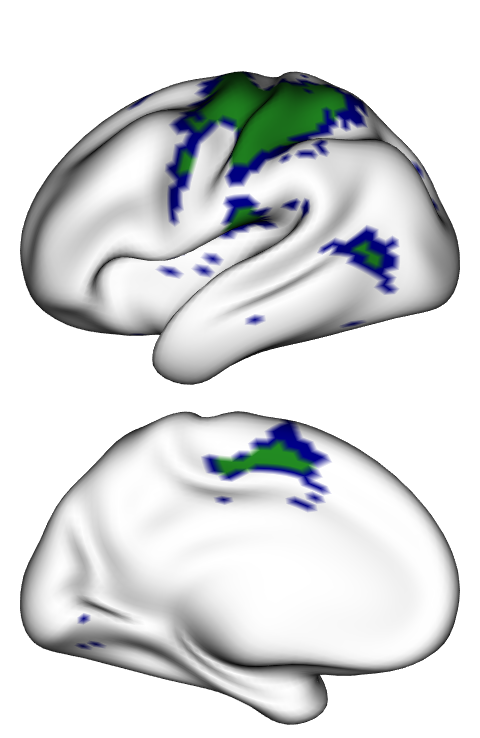
\includegraphics[width=1.5in]{plots/604_hand_classical_activation_map.png} \\ \hline
		\multicolumn{2}{c}{} & \multicolumn{2}{c}{\textcolor{MidnightBlue}{$\blacksquare$} FDR \textcolor{OliveGreen}{$\blacksquare$} FWER } & \multicolumn{1}{c}{} \\
	\end{tabularx}	

	\newpage
	
	\pagestyle{empty}

	\begin{figure}
		\begin{subfigure}{\textwidth}
			\begin{tabularx}{\textwidth}{|m{1em}|X|X|X|X|}
				\multicolumn{1}{c}{} & \multicolumn{1}{c}{\textbf{Visual Cue}} & \multicolumn{1}{c}{\textbf{Tongue}} & \multicolumn{1}{c}{\textbf{Right Foot}} & \multicolumn{1}{c}{\textbf{Right Hand}} \\ \hline
				\rotatebox{90}{\textbf{Bayesian GLM}}& 
				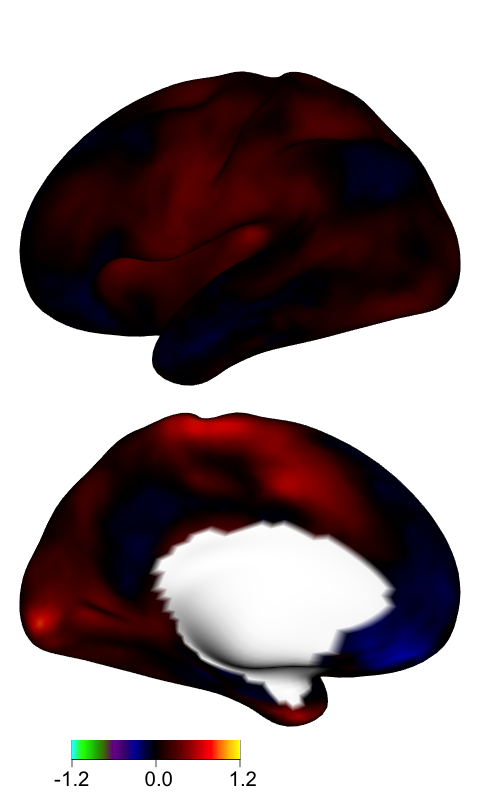
\includegraphics[width=0.2\textwidth]{plots/601_group_Bayes_visual_cue.png} &
				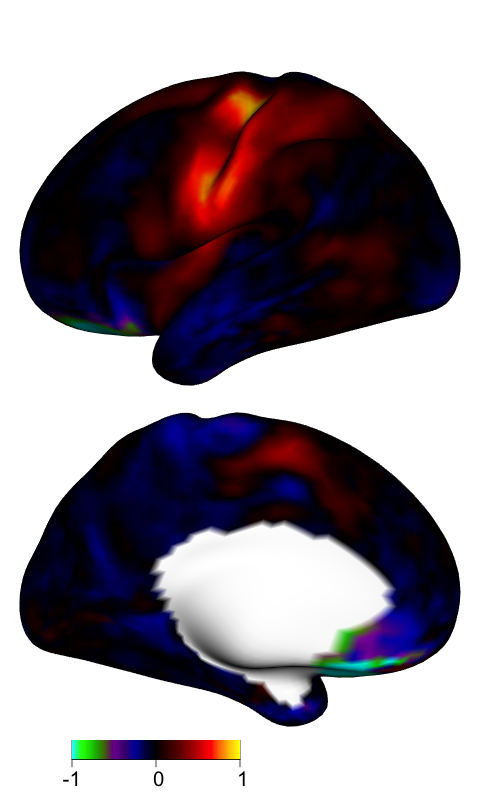
\includegraphics[width=0.2\textwidth]{plots/601_group_Bayes_tongue.png} &
				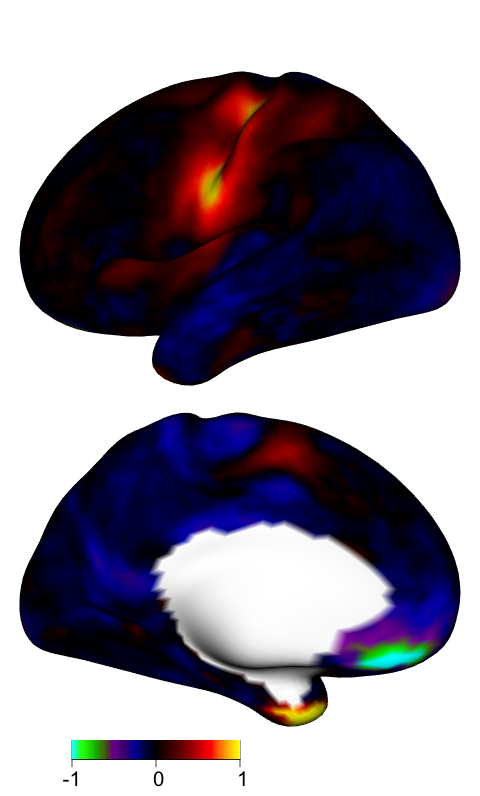
\includegraphics[width=0.2\textwidth]{plots/601_group_Bayes_right_foot.png} &
				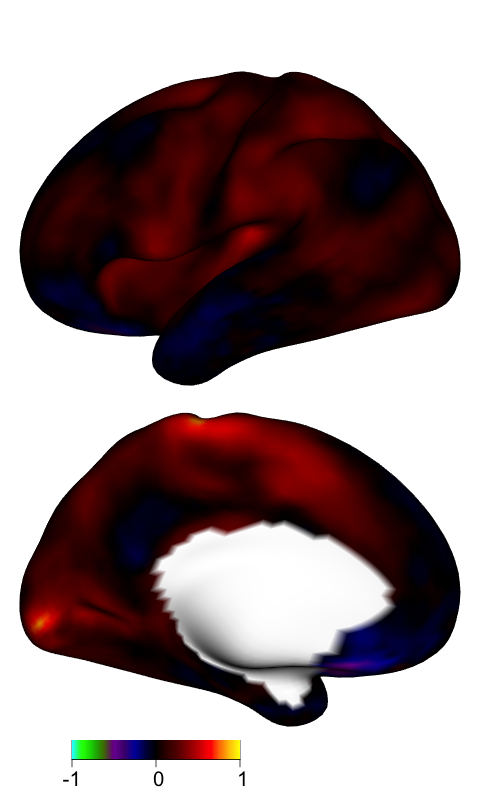
\includegraphics[width=0.2\textwidth]{plots/601_group_Bayes_right_hand.png} \\ \hline
				\rotatebox{90}{\textbf{Classical GLM}} & 
				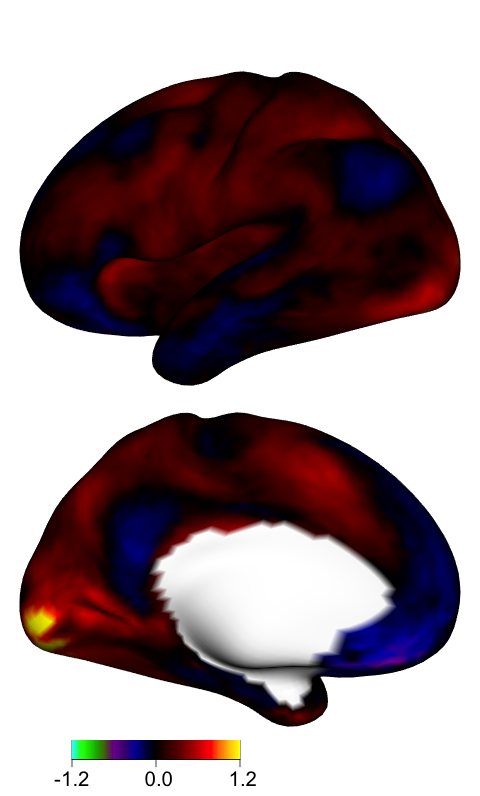
\includegraphics[width=0.2\textwidth]{plots/601_group_classical_visual_cue.png} &
				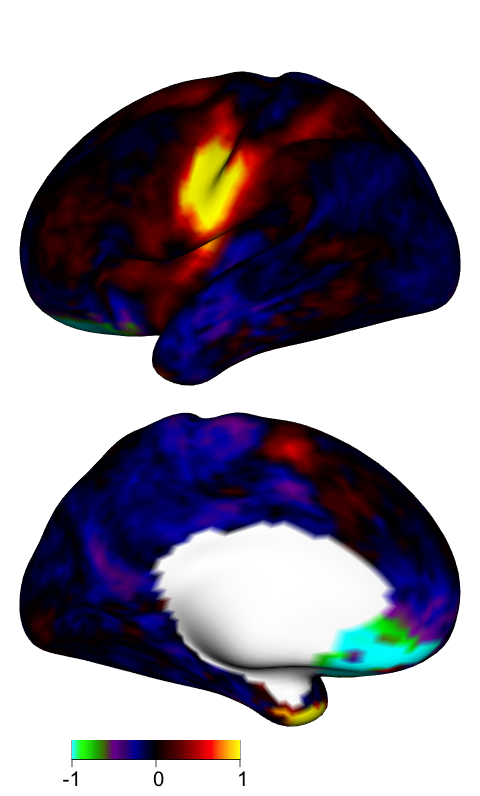
\includegraphics[width=0.2\textwidth]{plots/601_group_classical_tongue.png} &
				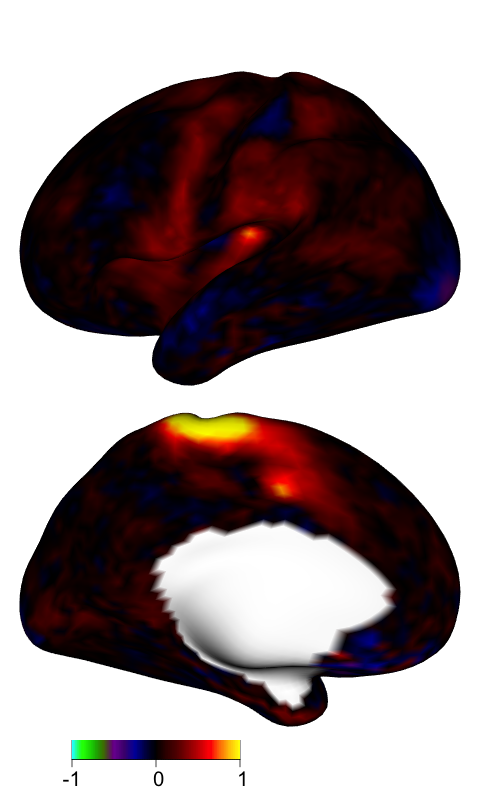
\includegraphics[width=0.2\textwidth]{plots/601_group_classical_right_foot.png} &
				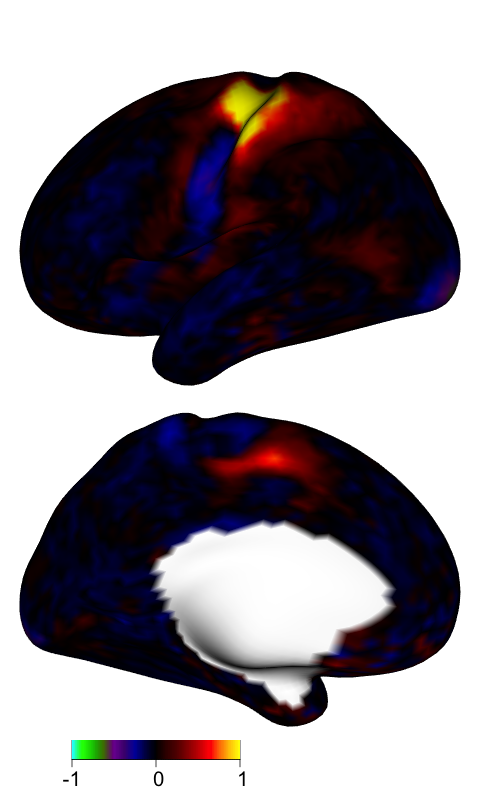
\includegraphics[width=0.2\textwidth]{plots/601_group_classical_right_hand.png} \\ \hline
			\end{tabularx}
		\caption{Estimates of activation amplitude in terms of percent signal change.}
		\label{subfig:group_est}
		\end{subfigure}
	
		\begin{subfigure}{\textwidth}
			\begin{tabularx}{\textwidth}{|m{1em}|X|X|X|X|}
				\hline
				\rotatebox{90}{\textbf{Bayesian GLM}}& 
				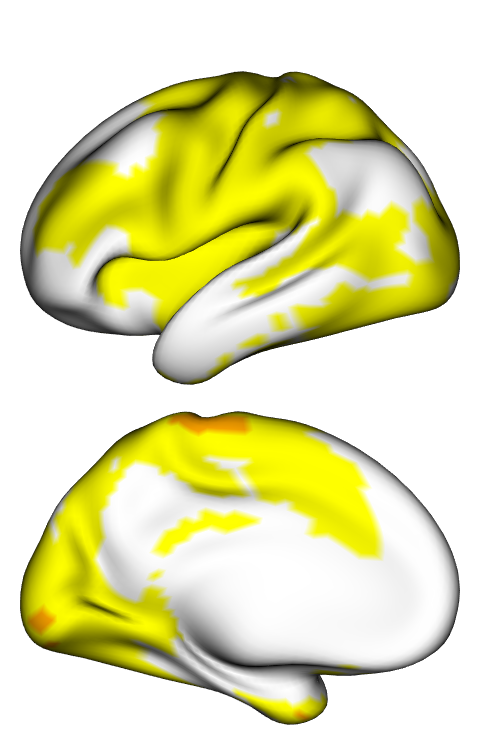
\includegraphics[width=0.2\textwidth]{plots/603_visual_cue_activation_map.png} &
				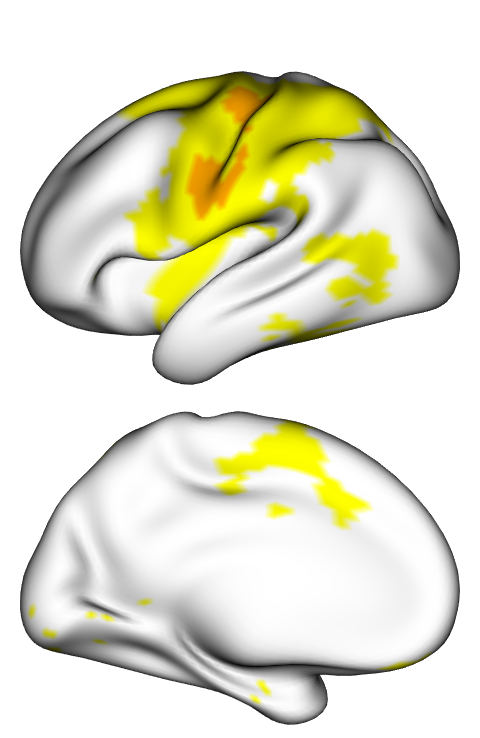
\includegraphics[width=0.2\textwidth]{plots/603_tongue_activation_map.png} &
				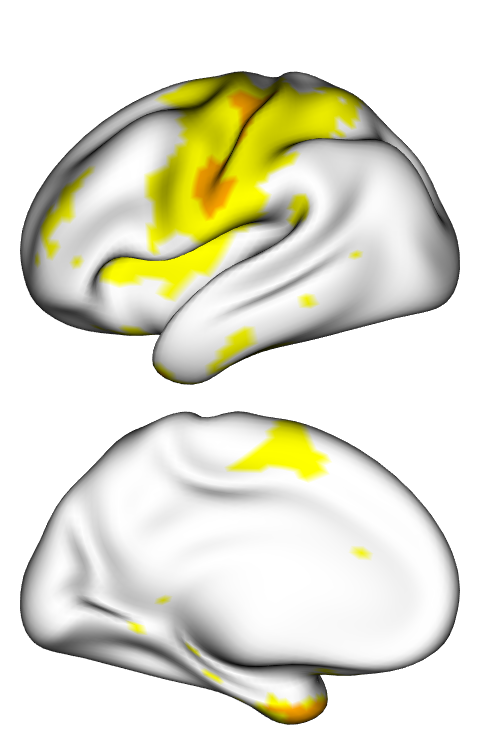
\includegraphics[width=0.2\textwidth]{plots/603_foot_activation_map.png} &
				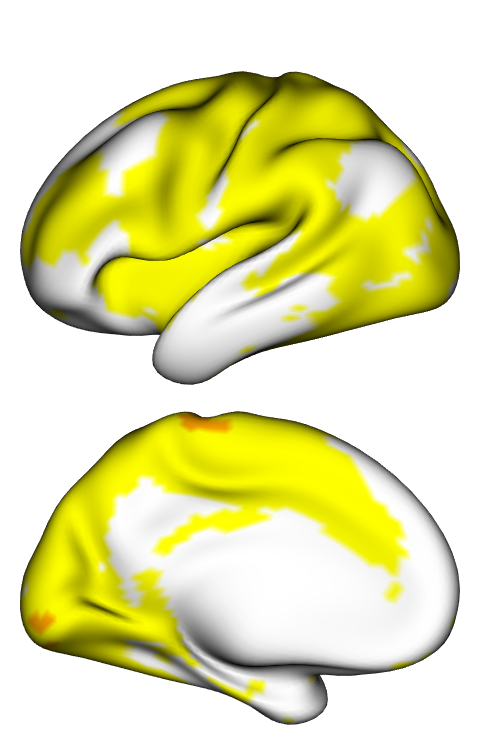
\includegraphics[width=0.2\textwidth]{plots/603_hand_activation_map.png} \\ \hline
				\multicolumn{2}{c}{} & \multicolumn{2}{c}{$\gamma = $ \textcolor{yellow}{$\blacksquare$} $0\%$ \textcolor{orange}{$\blacksquare$} $0.5\%$ } & \multicolumn{1}{c}{} \\ \hline
				\rotatebox{90}{\textbf{Classical GLM}} & 
				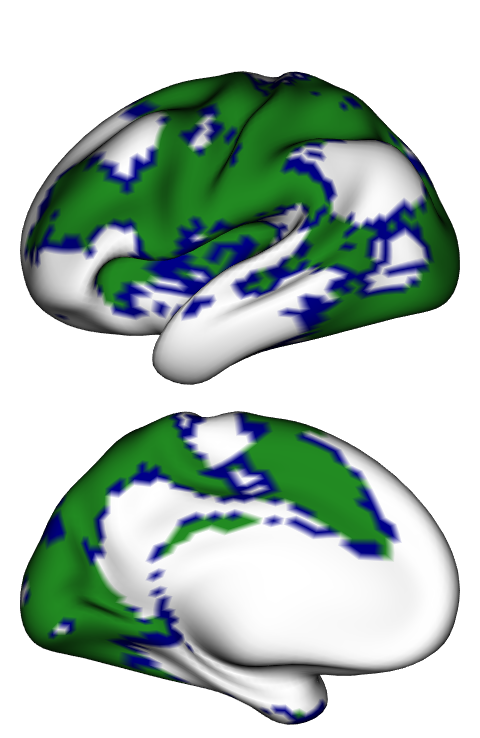
\includegraphics[width=0.2\textwidth]{plots/604_visual_cue_classical_activation_map.png} &
				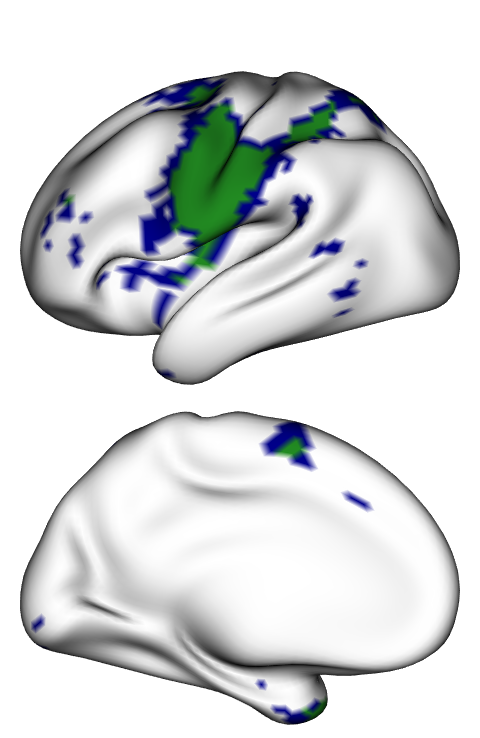
\includegraphics[width=0.2\textwidth]{plots/604_tongue_classical_activation_map.png} &
				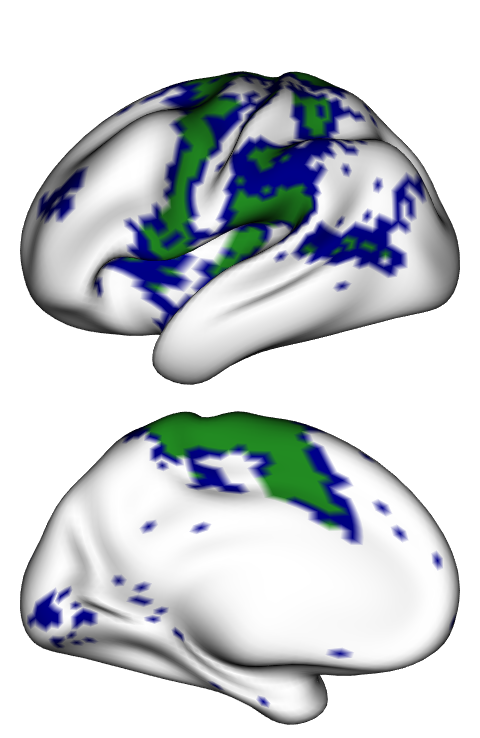
\includegraphics[width=0.2\textwidth]{plots/604_foot_classical_activation_map.png} &
				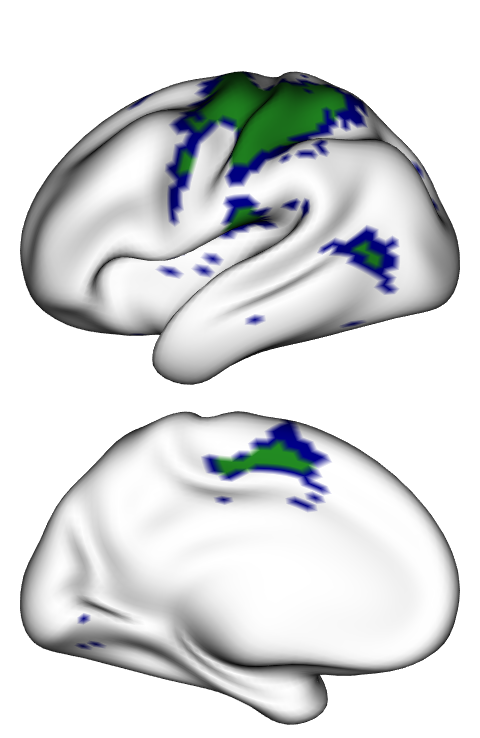
\includegraphics[width=0.2\textwidth]{plots/604_hand_classical_activation_map.png} \\ \hline
				\multicolumn{2}{c}{} & \multicolumn{2}{c}{\textcolor{Blue}{$\blacksquare$} FDR \textcolor{OliveGreen}{$\blacksquare$} FWER } & \multicolumn{1}{c}{} \\
			\end{tabularx}	
		\caption{Areas of activations based on the significance level $\alpha = 0.01$.}
		\label{subfig:group_act}
		\end{subfigure}
	\caption{Group-level estimates of activation amplitude (\ref{subfig:group_est}) and areas of activation (\ref{subfig:group_act}) for four tasks of the motor study. For the Bayesian GLM, the estimates displayed are group-level posterior means, and the areas of activation are based on two different activation thresholds $\gamma$ (0\% and 0.5\% local signal change.)}
	\label{fig:group_est_and_act}
	\end{figure}
	
	\newpage

	\section{Intraclass Correlation}
	
	\begin{figure}
		\begin{tabularx}{\textwidth}{|m{1em}|X|X|X|X|}
			\hline
			\rotatebox{90}{\textbf{Bayesian GLM}}& 
			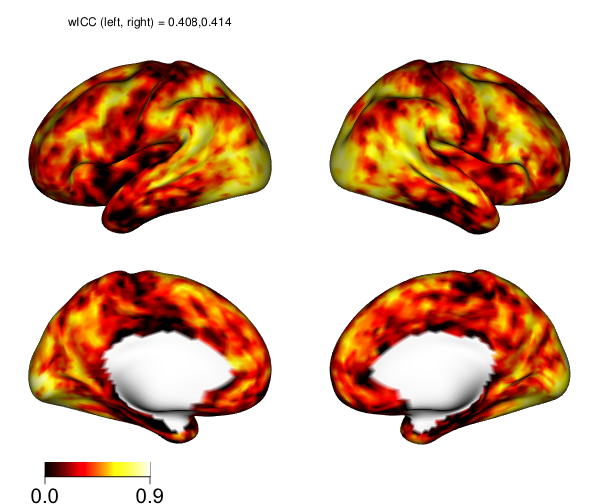
\includegraphics[width=0.2\textwidth]{plots/602_visual_cue_icc_bayesian_avg_left.png} &
			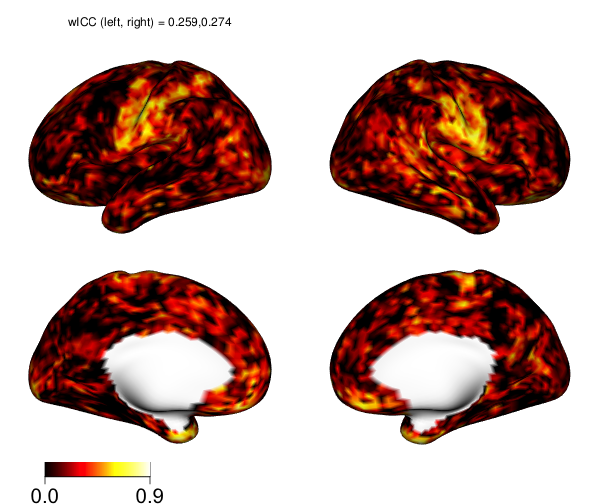
\includegraphics[width=0.2\textwidth]{plots/602_tongue_icc_bayesian_avg_left.png} &
			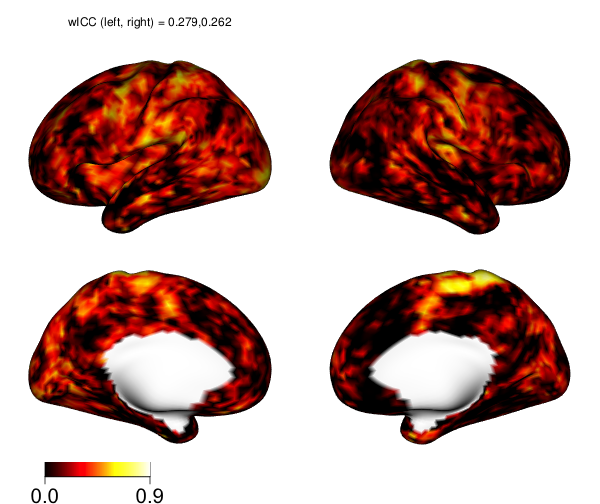
\includegraphics[width=0.2\textwidth]{plots/602_foot_icc_bayesian_avg_left.png} &
			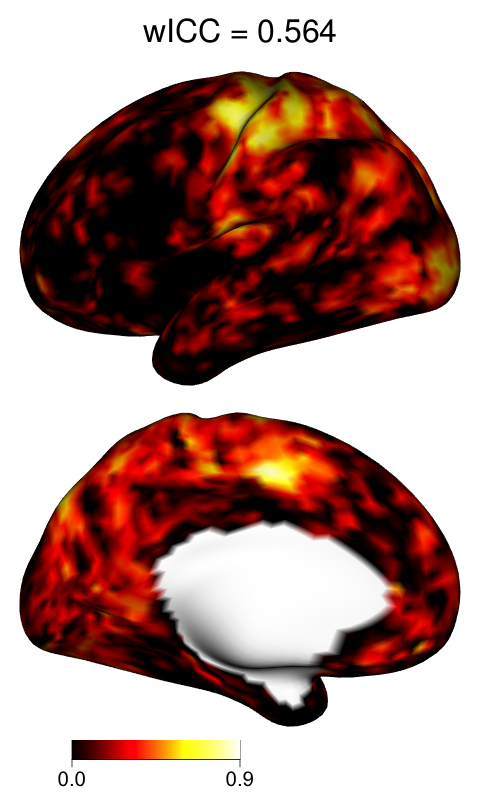
\includegraphics[width=0.2\textwidth]{plots/602_hand_icc_bayesian_avg_left.png} \\ \hline
			\rotatebox{90}{\textbf{Classical GLM}} & 
			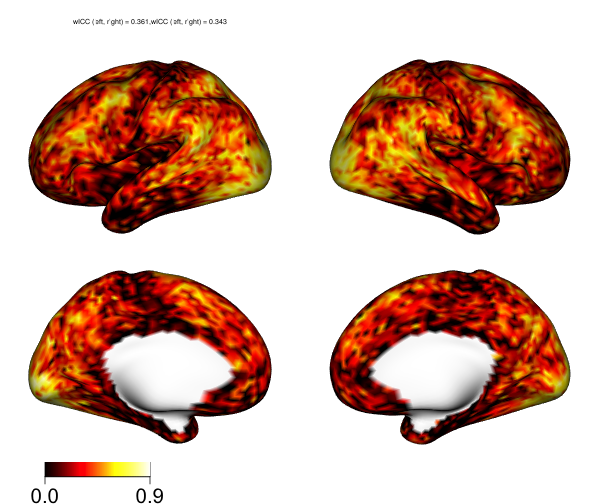
\includegraphics[width=0.2\textwidth]{plots/602_visual_cue_icc_classical_avg_left.png} &
			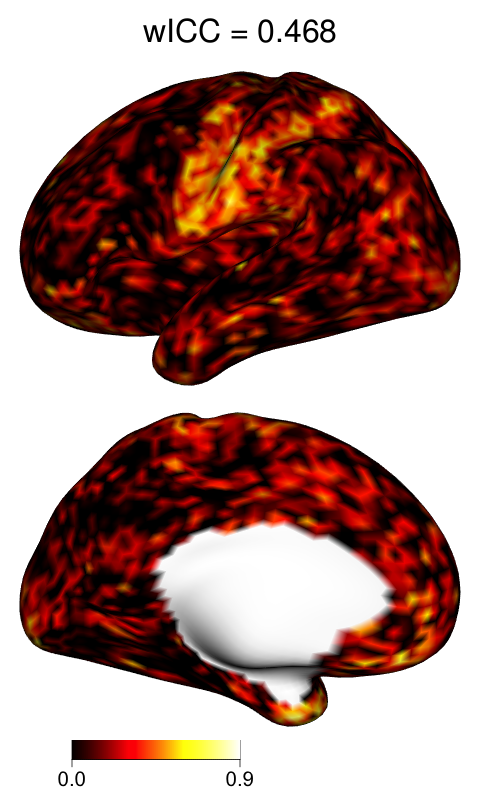
\includegraphics[width=0.2\textwidth]{plots/602_tongue_icc_classical_avg_left.png} &
			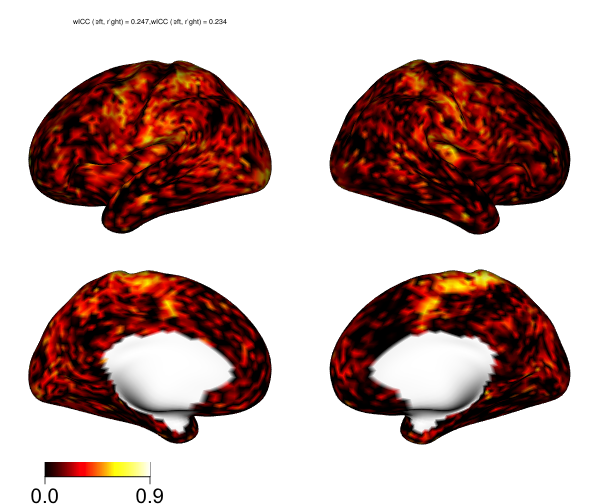
\includegraphics[width=0.2\textwidth]{plots/602_foot_icc_classical_avg_left.png} &
			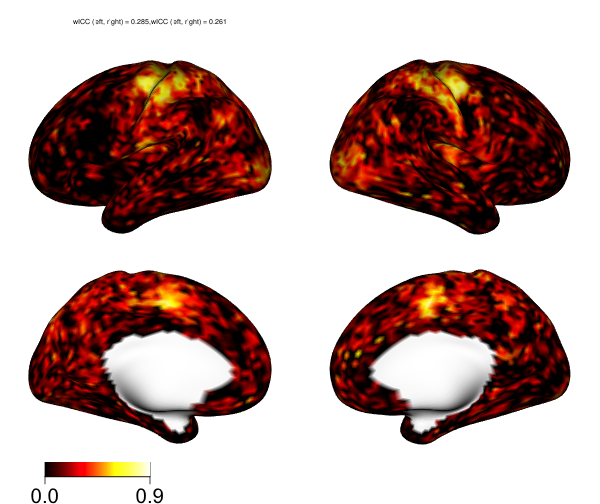
\includegraphics[width=0.2\textwidth]{plots/602_hand_icc_classical_avg_left.png} \\ \hline
		\end{tabularx}	
		\caption{Intraclass correlation coefficient (ICC) for the similarity of the average amplitude estimates across the two visits in the study data for the four motor tasks. Only the left hemisphere is shown due to space. The weighted ICC (wICC) is also shown as a metric to compare the images.}
		\label{fig:icc}
	\end{figure}

\end{document}